\begin{figure}[t]
	\begin{center}



    \tikzset{every picture/.style={line width=0.75pt}} %set default line width to 0.75pt        
    
    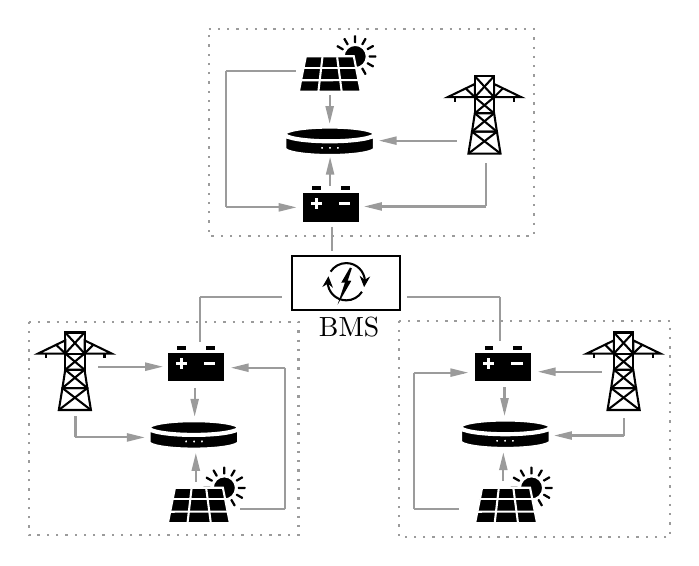
\begin{tikzpicture}[x=0.75pt,y=0.75pt,yscale=-1,xscale=1]
    %uncomment if require: \path (0,446); %set diagram left start at 0, and has height of 446
    
        %Shape: Ellipse [id:dp23689960204771032] 
        \draw  [color={rgb, 255:red, 255; green, 255; blue, 255 }  ,draw opacity=1 ][fill={rgb, 255:red, 0; green, 0; blue, 0 }  ,fill opacity=1 ] (155.38,17.72) .. controls (155.38,14.63) and (157.89,12.13) .. (160.97,12.13) .. controls (164.06,12.13) and (166.56,14.63) .. (166.56,17.72) .. controls (166.56,20.81) and (164.06,23.31) .. (160.97,23.31) .. controls (157.89,23.31) and (155.38,20.81) .. (155.38,17.72) -- cycle ;
        %Rounded Rect [id:dp7350954357882564] 
        \draw   (167.98,17.67) .. controls (167.98,17.66) and (167.99,17.65) .. (168,17.65) -- (170.69,17.65) .. controls (170.7,17.65) and (170.71,17.66) .. (170.71,17.67) -- (170.71,17.72) .. controls (170.71,17.73) and (170.7,17.74) .. (170.69,17.74) -- (168,17.74) .. controls (167.99,17.74) and (167.98,17.73) .. (167.98,17.72) -- cycle ;
        %Rounded Rect [id:dp5817858075714595] 
        \draw   (152.56,12.82) .. controls (152.57,12.81) and (152.58,12.8) .. (152.59,12.81) -- (154.92,14.16) .. controls (154.93,14.16) and (154.93,14.17) .. (154.93,14.18) -- (154.9,14.23) .. controls (154.89,14.24) and (154.88,14.24) .. (154.87,14.24) -- (152.54,12.89) .. controls (152.53,12.88) and (152.53,12.87) .. (152.53,12.86) -- cycle ;
        %Rounded Rect [id:dp562001902201841] 
        \draw   (155.9,9.37) .. controls (155.91,9.36) and (155.92,9.36) .. (155.92,9.37) -- (157.27,11.71) .. controls (157.27,11.71) and (157.27,11.72) .. (157.26,11.73) -- (157.22,11.76) .. controls (157.21,11.76) and (157.2,11.76) .. (157.19,11.75) -- (155.84,9.42) .. controls (155.84,9.41) and (155.84,9.4) .. (155.85,9.39) -- cycle ;
        %Rounded Rect [id:dp24994446560754513] 
        \draw   (160.96,8.01) .. controls (160.97,8.01) and (160.97,8.01) .. (160.97,8.02) -- (160.97,10.72) .. controls (160.97,10.73) and (160.97,10.74) .. (160.96,10.74) -- (160.9,10.74) .. controls (160.89,10.74) and (160.88,10.73) .. (160.88,10.72) -- (160.88,8.02) .. controls (160.88,8.01) and (160.89,8.01) .. (160.9,8.01) -- cycle ;
        %Rounded Rect [id:dp41080675695046875] 
        \draw   (151.26,17.65) .. controls (151.26,17.64) and (151.27,17.63) .. (151.28,17.63) -- (153.97,17.63) .. controls (153.98,17.63) and (153.99,17.64) .. (153.99,17.65) -- (153.99,17.7) .. controls (153.99,17.71) and (153.98,17.72) .. (153.97,17.72) -- (151.28,17.72) .. controls (151.27,17.72) and (151.26,17.71) .. (151.26,17.7) -- cycle ;
        %Rounded Rect [id:dp2589224672963768] 
        \draw   (164.51,23.63) .. controls (164.52,23.63) and (164.53,23.63) .. (164.54,23.64) -- (165.88,25.97) .. controls (165.89,25.98) and (165.89,25.99) .. (165.88,26) -- (165.83,26.02) .. controls (165.82,26.03) and (165.81,26.03) .. (165.8,26.02) -- (164.46,23.68) .. controls (164.45,23.68) and (164.46,23.66) .. (164.46,23.66) -- cycle ;
        %Rounded Rect [id:dp52965196080424] 
        \draw   (161.05,24.71) .. controls (161.06,24.71) and (161.06,24.72) .. (161.06,24.73) -- (161.06,27.42) .. controls (161.06,27.43) and (161.06,27.44) .. (161.05,27.44) -- (160.99,27.44) .. controls (160.98,27.44) and (160.97,27.43) .. (160.97,27.42) -- (160.97,24.73) .. controls (160.97,24.72) and (160.98,24.71) .. (160.99,24.71) -- cycle ;
        %Rounded Rect [id:dp4402538190695453] 
        \draw   (167.1,21.03) .. controls (167.1,21.02) and (167.11,21.01) .. (167.12,21.02) -- (169.46,22.37) .. controls (169.46,22.37) and (169.47,22.38) .. (169.46,22.39) -- (169.43,22.44) .. controls (169.43,22.45) and (169.42,22.45) .. (169.41,22.45) -- (167.08,21.1) .. controls (167.07,21.09) and (167.07,21.08) .. (167.07,21.07) -- cycle ;
        %Rounded Rect [id:dp6996007283347523] 
        \draw   (165.88,9.36) .. controls (165.89,9.36) and (165.89,9.37) .. (165.88,9.38) -- (164.54,11.71) .. controls (164.53,11.72) and (164.52,11.73) .. (164.51,11.72) -- (164.46,11.69) .. controls (164.46,11.69) and (164.45,11.68) .. (164.46,11.67) -- (165.8,9.34) .. controls (165.81,9.33) and (165.82,9.32) .. (165.83,9.33) -- cycle ;
        %Rounded Rect [id:dp670060683107357] 
        \draw   (169.46,12.74) .. controls (169.47,12.75) and (169.46,12.76) .. (169.46,12.77) -- (167.12,14.11) .. controls (167.11,14.12) and (167.1,14.12) .. (167.1,14.11) -- (167.07,14.06) .. controls (167.07,14.05) and (167.07,14.04) .. (167.08,14.03) -- (169.41,12.69) .. controls (169.42,12.68) and (169.43,12.69) .. (169.43,12.69) -- cycle ;
        %Rounded Rect [id:dp17906894780647287] 
        \draw   (154.93,20.95) .. controls (154.93,20.96) and (154.93,20.97) .. (154.92,20.98) -- (152.59,22.32) .. controls (152.58,22.33) and (152.57,22.33) .. (152.56,22.32) -- (152.53,22.27) .. controls (152.53,22.26) and (152.53,22.25) .. (152.54,22.24) -- (154.87,20.9) .. controls (154.88,20.89) and (154.89,20.9) .. (154.9,20.9) -- cycle ;
        %Rounded Rect [id:dp7163585653714504] 
        \draw   (157.13,23.62) .. controls (157.14,23.63) and (157.14,23.64) .. (157.13,23.65) -- (155.79,25.98) .. controls (155.78,25.99) and (155.77,25.99) .. (155.76,25.99) -- (155.72,25.96) .. controls (155.71,25.95) and (155.7,25.94) .. (155.71,25.94) -- (157.06,23.6) .. controls (157.06,23.59) and (157.07,23.59) .. (157.08,23.6) -- cycle ;
        
        %Shape: Trapezoid [id:dp39839281755362443] 
        \draw  [color={rgb, 255:red, 255; green, 255; blue, 255 }  ,draw opacity=1 ][fill={rgb, 255:red, 0; green, 0; blue, 0 }  ,fill opacity=1 ] (133.8,34.68) -- (137.2,17.61) -- (160.28,17.61) -- (163.68,34.68) -- cycle ;
        %Straight Lines [id:da8047810174415737] 
        \draw [color={rgb, 255:red, 255; green, 255; blue, 255 }  ,draw opacity=1 ][fill={rgb, 255:red, 0; green, 0; blue, 0 }  ,fill opacity=1 ]   (135.05,29.17) -- (162.64,29.12) ;
        %Straight Lines [id:da8343675725090776] 
        \draw [color={rgb, 255:red, 255; green, 255; blue, 255 }  ,draw opacity=1 ][fill={rgb, 255:red, 0; green, 0; blue, 0 }  ,fill opacity=1 ]   (136,23.22) -- (161.09,23.22) ;
        %Straight Lines [id:da6746426481591967] 
        \draw [color={rgb, 255:red, 255; green, 255; blue, 255 }  ,draw opacity=1 ][fill={rgb, 255:red, 0; green, 0; blue, 0 }  ,fill opacity=1 ]   (152.28,18.1) -- (154.51,34.94) ;
        %Straight Lines [id:da546227329864996] 
        \draw [color={rgb, 255:red, 255; green, 255; blue, 255 }  ,draw opacity=1 ][fill={rgb, 255:red, 0; green, 0; blue, 0 }  ,fill opacity=1 ]   (145.19,17.94) -- (143.19,35.06) ;
        
        
        %Shape: Can [id:dp9005011599408153] 
        \draw  [color={rgb, 255:red, 255; green, 255; blue, 255 }  ,draw opacity=1 ][fill={rgb, 255:red, 0; green, 0; blue, 0 }  ,fill opacity=1 ][line width=1.5]  (170.53,55.02) -- (170.53,62.12) .. controls (170.53,64.08) and (160.74,65.67) .. (148.67,65.67) .. controls (136.6,65.67) and (126.82,64.08) .. (126.82,62.12) -- (126.82,55.02) .. controls (126.82,53.06) and (136.6,51.47) .. (148.67,51.47) .. controls (160.74,51.47) and (170.53,53.06) .. (170.53,55.02) .. controls (170.53,56.98) and (160.74,58.57) .. (148.67,58.57) .. controls (136.6,58.57) and (126.82,56.98) .. (126.82,55.02) ;
        %Shape: Ellipse [id:dp627980002725933] 
        \draw  [fill={rgb, 255:red, 255; green, 255; blue, 255 }  ,fill opacity=1 ] (147.75,61.72) .. controls (147.75,61.13) and (148.23,60.65) .. (148.82,60.65) .. controls (149.41,60.65) and (149.89,61.13) .. (149.89,61.72) .. controls (149.89,62.31) and (149.41,62.79) .. (148.82,62.79) .. controls (148.23,62.79) and (147.75,62.31) .. (147.75,61.72) -- cycle ;
        %Shape: Ellipse [id:dp32022930297328456] 
        \draw  [fill={rgb, 255:red, 255; green, 255; blue, 255 }  ,fill opacity=1 ] (151.55,61.72) .. controls (151.55,61.13) and (152.02,60.65) .. (152.62,60.65) .. controls (153.21,60.65) and (153.68,61.13) .. (153.68,61.72) .. controls (153.68,62.31) and (153.21,62.79) .. (152.62,62.79) .. controls (152.02,62.79) and (151.55,62.31) .. (151.55,61.72) -- cycle ;
        %Shape: Ellipse [id:dp09464548947851847] 
        \draw  [fill={rgb, 255:red, 255; green, 255; blue, 255 }  ,fill opacity=1 ] (143.96,61.72) .. controls (143.96,61.13) and (144.44,60.65) .. (145.03,60.65) .. controls (145.62,60.65) and (146.1,61.13) .. (146.1,61.72) .. controls (146.1,62.31) and (145.62,62.79) .. (145.03,62.79) .. controls (144.44,62.79) and (143.96,62.31) .. (143.96,61.72) -- cycle ;
        
        %Shape: Rectangle [id:dp35865913094459034] 
        \draw  [fill={rgb, 255:red, 0; green, 0; blue, 0 }  ,fill opacity=1 ] (136.18,83.97) -- (162.32,83.97) -- (162.32,96.73) -- (136.18,96.73) -- cycle ;
        %Shape: Cross [id:dp9459558747780203] 
        \draw  [fill={rgb, 255:red, 255; green, 255; blue, 255 }  ,fill opacity=1 ] (143.64,85.38) -- (140.99,85.38) -- (140.99,87.25) -- (139.12,87.25) -- (139.12,89.9) -- (140.99,89.9) -- (140.99,91.76) -- (143.64,91.76) -- (143.64,89.9) -- (145.51,89.9) -- (145.51,87.25) -- (143.64,87.25) -- cycle ;
        %Shape: Rectangle [id:dp8159450856522705] 
        \draw  [fill={rgb, 255:red, 255; green, 255; blue, 255 }  ,fill opacity=1 ] (152.74,87.11) -- (159.17,87.11) -- (159.17,89.98) -- (152.74,89.98) -- cycle ;
        %Shape: Rectangle [id:dp9559476182094357] 
        \draw  [fill={rgb, 255:red, 0; green, 0; blue, 0 }  ,fill opacity=1 ] (140.83,80.67) -- (144.1,80.67) -- (144.1,81.66) -- (140.83,81.66) -- cycle ;
        %Shape: Rectangle [id:dp06489231659707517] 
        \draw  [fill={rgb, 255:red, 0; green, 0; blue, 0 }  ,fill opacity=1 ] (154.7,80.67) -- (157.96,80.67) -- (157.96,81.66) -- (154.7,81.66) -- cycle ;
        
        %Shape: Trapezoid [id:dp5856244719833053] 
        \draw   (215.52,64.5) -- (217.25,53.93) -- (229.25,53.93) -- (230.98,64.5) -- cycle ;
        %Shape: Trapezoid [id:dp44335621565613703] 
        \draw   (217.25,53.93) -- (218.6,45.09) -- (227.9,45.09) -- (229.25,53.93) -- cycle ;
        %Shape: Trapezoid [id:dp2690273077646286] 
        \draw   (218.6,45.09) -- (218.6,37.3) -- (227.9,37.3) -- (227.9,45.09) -- cycle ;
        %Shape: Trapezoid [id:dp789123773409603] 
        \draw   (218.6,37.3) -- (218.6,27.17) -- (227.9,27.17) -- (227.9,37.3) -- cycle ;
        %Straight Lines [id:da828316850046003] 
        \draw    (217.25,53.93) -- (230.98,64.5) ;
        %Straight Lines [id:da591569368482918] 
        \draw    (215.52,64.5) -- (229.25,53.93) ;
        %Straight Lines [id:da7192792870901867] 
        \draw    (217.25,53.93) -- (227.9,45.09) ;
        %Straight Lines [id:da25942426045741995] 
        \draw    (229.25,53.93) -- (218.6,45.09) ;
        %Straight Lines [id:da998802426261975] 
        \draw    (227.9,45.09) -- (218.6,37.3) ;
        %Straight Lines [id:da38916705477465796] 
        \draw    (218.6,45.09) -- (227.9,37.3) ;
        %Straight Lines [id:da26657305293991884] 
        \draw    (218.6,37.3) -- (227.9,27.17) ;
        %Straight Lines [id:da31720929903327444] 
        \draw    (227.9,37.3) -- (218.6,27.17) ;
        %Shape: Right Triangle [id:dp46306371951470315] 
        \draw   (227.9,30.97) -- (240.97,37.3) -- (227.9,37.3) -- cycle ;
        %Straight Lines [id:da5846990799110421] 
        \draw    (227.9,37.3) -- (232.18,33.03) ;
        %Straight Lines [id:da9958530803374206] 
        \draw    (237.52,37.43) -- (237.52,39.57) ;
        
        %Shape: Right Triangle [id:dp09576900324503912] 
        \draw   (218.6,30.97) -- (205.53,37.3) -- (218.6,37.3) -- cycle ;
        %Straight Lines [id:da10297154407621023] 
        \draw    (214.45,33.3) -- (218.6,37.3) ;
        %Straight Lines [id:da9008160700393986] 
        \draw    (209.12,37.43) -- (209.12,39.57) ;
        
        %Straight Lines [id:da3670426702577094] 
        \draw [color={rgb, 255:red, 155; green, 155; blue, 155 }  ,draw opacity=1 ]   (224,89.97) -- (224,69.11) ;
        %Straight Lines [id:da3081807630858884] 
        \draw [color={rgb, 255:red, 155; green, 155; blue, 155 }  ,draw opacity=1 ]   (98.67,24.9) -- (132.5,24.9) ;
        %Straight Lines [id:da9003194521232087] 
        \draw [color={rgb, 255:red, 155; green, 155; blue, 155 }  ,draw opacity=1 ]   (98.67,24.9) -- (98.67,90.4) ;
        %Straight Lines [id:da9853775896451256] 
        \draw [color={rgb, 255:red, 155; green, 155; blue, 155 }  ,draw opacity=1 ]   (98.67,90.4) -- (130.5,90.4) ;
        \draw [shift={(132.5,90.4)}, rotate = 180] [fill={rgb, 255:red, 155; green, 155; blue, 155 }  ,fill opacity=1 ][line width=0.08]  [draw opacity=0] (8.4,-2.1) -- (0,0) -- (8.4,2.1) -- cycle    ;
        %Straight Lines [id:da9683252488589866] 
        \draw [color={rgb, 255:red, 155; green, 155; blue, 155 }  ,draw opacity=1 ]   (148.86,79.97) -- (148.86,68.26) ;
        \draw [shift={(148.86,66.26)}, rotate = 90] [fill={rgb, 255:red, 155; green, 155; blue, 155 }  ,fill opacity=1 ][line width=0.08]  [draw opacity=0] (8.4,-2.1) -- (0,0) -- (8.4,2.1) -- cycle    ;
        %Straight Lines [id:da6427138667449821] 
        \draw [color={rgb, 255:red, 155; green, 155; blue, 155 }  ,draw opacity=1 ]   (148.67,36.26) -- (148.67,47.97) ;
        \draw [shift={(148.67,49.97)}, rotate = 270] [fill={rgb, 255:red, 155; green, 155; blue, 155 }  ,fill opacity=1 ][line width=0.08]  [draw opacity=0] (8.4,-2.1) -- (0,0) -- (8.4,2.1) -- cycle    ;
        %Straight Lines [id:da8819546339421043] 
        \draw [color={rgb, 255:red, 155; green, 155; blue, 155 }  ,draw opacity=1 ]   (210,58.26) -- (174.57,58.26) ;
        \draw [shift={(172.57,58.26)}, rotate = 360] [fill={rgb, 255:red, 155; green, 155; blue, 155 }  ,fill opacity=1 ][line width=0.08]  [draw opacity=0] (8.4,-2.1) -- (0,0) -- (8.4,2.1) -- cycle    ;
        %Straight Lines [id:da12696545096661116] 
        \draw [color={rgb, 255:red, 155; green, 155; blue, 155 }  ,draw opacity=1 ]   (224,89.97) -- (167.43,89.97) ;
        \draw [shift={(165.43,89.97)}, rotate = 360] [fill={rgb, 255:red, 155; green, 155; blue, 155 }  ,fill opacity=1 ][line width=0.08]  [draw opacity=0] (8.4,-2.1) -- (0,0) -- (8.4,2.1) -- cycle    ;
        
        %Shape: Ellipse [id:dp046440233113860696] 
        \draw  [color={rgb, 255:red, 255; green, 255; blue, 255 }  ,draw opacity=1 ][fill={rgb, 255:red, 0; green, 0; blue, 0 }  ,fill opacity=1 ] (92.32,225.59) .. controls (92.32,222.5) and (94.82,220) .. (97.91,220) .. controls (100.99,220) and (103.5,222.5) .. (103.5,225.59) .. controls (103.5,228.68) and (100.99,231.18) .. (97.91,231.18) .. controls (94.82,231.18) and (92.32,228.68) .. (92.32,225.59) -- cycle ;
        %Rounded Rect [id:dp21673028923709814] 
        \draw   (104.91,225.53) .. controls (104.91,225.52) and (104.92,225.52) .. (104.93,225.52) -- (107.62,225.52) .. controls (107.63,225.52) and (107.64,225.52) .. (107.64,225.53) -- (107.64,225.59) .. controls (107.64,225.6) and (107.63,225.61) .. (107.62,225.61) -- (104.93,225.61) .. controls (104.92,225.61) and (104.91,225.6) .. (104.91,225.59) -- cycle ;
        %Rounded Rect [id:dp9417842391430391] 
        \draw   (89.5,220.68) .. controls (89.5,220.67) and (89.51,220.67) .. (89.52,220.68) -- (91.85,222.02) .. controls (91.86,222.03) and (91.86,222.04) .. (91.86,222.05) -- (91.83,222.1) .. controls (91.83,222.1) and (91.82,222.11) .. (91.81,222.1) -- (89.47,220.75) .. controls (89.47,220.75) and (89.46,220.74) .. (89.47,220.73) -- cycle ;
        %Rounded Rect [id:dp4967499642080284] 
        \draw   (92.83,217.23) .. controls (92.84,217.23) and (92.85,217.23) .. (92.86,217.24) -- (94.2,219.57) .. controls (94.21,219.58) and (94.2,219.59) .. (94.2,219.6) -- (94.15,219.62) .. controls (94.14,219.63) and (94.13,219.63) .. (94.12,219.62) -- (92.78,217.28) .. controls (92.77,217.28) and (92.78,217.26) .. (92.78,217.26) -- cycle ;
        %Rounded Rect [id:dp42182766171645003] 
        \draw   (97.89,215.87) .. controls (97.9,215.87) and (97.91,215.88) .. (97.91,215.89) -- (97.91,218.58) .. controls (97.91,218.59) and (97.9,218.6) .. (97.89,218.6) -- (97.83,218.6) .. controls (97.82,218.6) and (97.82,218.59) .. (97.82,218.58) -- (97.82,215.89) .. controls (97.82,215.88) and (97.82,215.87) .. (97.83,215.87) -- cycle ;
        %Rounded Rect [id:dp7372953483874027] 
        \draw   (88.19,225.52) .. controls (88.19,225.51) and (88.2,225.5) .. (88.21,225.5) -- (90.9,225.5) .. controls (90.91,225.5) and (90.92,225.51) .. (90.92,225.52) -- (90.92,225.57) .. controls (90.92,225.58) and (90.91,225.59) .. (90.9,225.59) -- (88.21,225.59) .. controls (88.2,225.59) and (88.19,225.58) .. (88.19,225.57) -- cycle ;
        %Rounded Rect [id:dp016554811734768915] 
        \draw   (101.44,231.5) .. controls (101.45,231.49) and (101.46,231.5) .. (101.47,231.51) -- (102.82,233.84) .. controls (102.82,233.85) and (102.82,233.86) .. (102.81,233.86) -- (102.76,233.89) .. controls (102.75,233.9) and (102.74,233.89) .. (102.74,233.88) -- (101.39,231.55) .. controls (101.39,231.54) and (101.39,231.53) .. (101.4,231.53) -- cycle ;
        %Rounded Rect [id:dp3333806907098691] 
        \draw   (97.98,232.57) .. controls (97.99,232.57) and (98,232.58) .. (98,232.59) -- (98,235.29) .. controls (98,235.3) and (97.99,235.3) .. (97.98,235.3) -- (97.92,235.3) .. controls (97.91,235.3) and (97.91,235.3) .. (97.91,235.29) -- (97.91,232.59) .. controls (97.91,232.58) and (97.91,232.57) .. (97.92,232.57) -- cycle ;
        %Rounded Rect [id:dp4045437830291596] 
        \draw   (104.03,228.89) .. controls (104.04,228.88) and (104.05,228.88) .. (104.06,228.89) -- (106.39,230.23) .. controls (106.4,230.24) and (106.4,230.25) .. (106.4,230.26) -- (106.37,230.31) .. controls (106.36,230.31) and (106.35,230.32) .. (106.34,230.31) -- (104.01,228.96) .. controls (104,228.96) and (104,228.95) .. (104,228.94) -- cycle ;
        %Rounded Rect [id:dp18140925314320766] 
        \draw   (102.81,217.22) .. controls (102.82,217.23) and (102.82,217.24) .. (102.82,217.25) -- (101.47,219.58) .. controls (101.46,219.59) and (101.45,219.59) .. (101.44,219.59) -- (101.4,219.56) .. controls (101.39,219.56) and (101.39,219.54) .. (101.39,219.54) -- (102.74,217.2) .. controls (102.74,217.19) and (102.75,217.19) .. (102.76,217.2) -- cycle ;
        %Rounded Rect [id:dp6960166673215535] 
        \draw   (106.4,220.61) .. controls (106.4,220.62) and (106.4,220.63) .. (106.39,220.63) -- (104.06,221.98) .. controls (104.05,221.98) and (104.04,221.98) .. (104.03,221.97) -- (104,221.93) .. controls (104,221.92) and (104,221.91) .. (104.01,221.9) -- (106.34,220.55) .. controls (106.35,220.55) and (106.36,220.55) .. (106.37,220.56) -- cycle ;
        %Rounded Rect [id:dp34185776666936607] 
        \draw   (91.86,228.82) .. controls (91.86,228.83) and (91.86,228.84) .. (91.85,228.84) -- (89.52,230.19) .. controls (89.51,230.19) and (89.5,230.19) .. (89.5,230.18) -- (89.47,230.14) .. controls (89.46,230.13) and (89.47,230.12) .. (89.47,230.11) -- (91.81,228.76) .. controls (91.82,228.76) and (91.83,228.76) .. (91.83,228.77) -- cycle ;
        %Rounded Rect [id:dp5556414628284645] 
        \draw   (94.06,231.49) .. controls (94.07,231.49) and (94.07,231.51) .. (94.07,231.51) -- (92.72,233.85) .. controls (92.72,233.86) and (92.71,233.86) .. (92.7,233.85) -- (92.65,233.83) .. controls (92.64,233.82) and (92.64,233.81) .. (92.64,233.8) -- (93.99,231.47) .. controls (93.99,231.46) and (94.01,231.46) .. (94.01,231.46) -- cycle ;
        
        %Shape: Trapezoid [id:dp9078658261484358] 
        \draw  [color={rgb, 255:red, 255; green, 255; blue, 255 }  ,draw opacity=1 ][fill={rgb, 255:red, 0; green, 0; blue, 0 }  ,fill opacity=1 ] (70.73,242.55) -- (74.13,225.48) -- (97.21,225.48) -- (100.61,242.55) -- cycle ;
        %Straight Lines [id:da6538397825350515] 
        \draw [color={rgb, 255:red, 255; green, 255; blue, 255 }  ,draw opacity=1 ][fill={rgb, 255:red, 0; green, 0; blue, 0 }  ,fill opacity=1 ]   (71.98,237.04) -- (99.58,236.99) ;
        %Straight Lines [id:da5435454566868603] 
        \draw [color={rgb, 255:red, 255; green, 255; blue, 255 }  ,draw opacity=1 ][fill={rgb, 255:red, 0; green, 0; blue, 0 }  ,fill opacity=1 ]   (72.94,231.09) -- (98.02,231.09) ;
        %Straight Lines [id:da24497164177888142] 
        \draw [color={rgb, 255:red, 255; green, 255; blue, 255 }  ,draw opacity=1 ][fill={rgb, 255:red, 0; green, 0; blue, 0 }  ,fill opacity=1 ]   (89.21,225.97) -- (91.45,242.81) ;
        %Straight Lines [id:da32161055867429855] 
        \draw [color={rgb, 255:red, 255; green, 255; blue, 255 }  ,draw opacity=1 ][fill={rgb, 255:red, 0; green, 0; blue, 0 }  ,fill opacity=1 ]   (82.13,225.81) -- (80.13,242.93) ;
        
        
        %Shape: Can [id:dp4496626078631891] 
        \draw  [color={rgb, 255:red, 255; green, 255; blue, 255 }  ,draw opacity=1 ][fill={rgb, 255:red, 0; green, 0; blue, 0 }  ,fill opacity=1 ][line width=1.5]  (105.06,196.49) -- (105.06,203.59) .. controls (105.06,205.55) and (95.28,207.14) .. (83.21,207.14) .. controls (71.14,207.14) and (61.35,205.55) .. (61.35,203.59) -- (61.35,196.49) .. controls (61.35,194.53) and (71.14,192.94) .. (83.21,192.94) .. controls (95.28,192.94) and (105.06,194.53) .. (105.06,196.49) .. controls (105.06,198.45) and (95.28,200.04) .. (83.21,200.04) .. controls (71.14,200.04) and (61.35,198.45) .. (61.35,196.49) ;
        %Shape: Ellipse [id:dp6589498088673775] 
        \draw  [fill={rgb, 255:red, 255; green, 255; blue, 255 }  ,fill opacity=1 ] (82.29,203.19) .. controls (82.29,202.6) and (82.76,202.12) .. (83.36,202.12) .. controls (83.95,202.12) and (84.43,202.6) .. (84.43,203.19) .. controls (84.43,203.78) and (83.95,204.26) .. (83.36,204.26) .. controls (82.76,204.26) and (82.29,203.78) .. (82.29,203.19) -- cycle ;
        %Shape: Ellipse [id:dp09849771978532496] 
        \draw  [fill={rgb, 255:red, 255; green, 255; blue, 255 }  ,fill opacity=1 ] (86.08,203.19) .. controls (86.08,202.6) and (86.56,202.12) .. (87.15,202.12) .. controls (87.74,202.12) and (88.22,202.6) .. (88.22,203.19) .. controls (88.22,203.78) and (87.74,204.26) .. (87.15,204.26) .. controls (86.56,204.26) and (86.08,203.78) .. (86.08,203.19) -- cycle ;
        %Shape: Ellipse [id:dp9620130396250384] 
        \draw  [fill={rgb, 255:red, 255; green, 255; blue, 255 }  ,fill opacity=1 ] (78.49,203.19) .. controls (78.49,202.6) and (78.97,202.12) .. (79.56,202.12) .. controls (80.15,202.12) and (80.63,202.6) .. (80.63,203.19) .. controls (80.63,203.78) and (80.15,204.26) .. (79.56,204.26) .. controls (78.97,204.26) and (78.49,203.78) .. (78.49,203.19) -- cycle ;
        
        %Shape: Rectangle [id:dp8525312211512277] 
        \draw  [fill={rgb, 255:red, 0; green, 0; blue, 0 }  ,fill opacity=1 ] (71.11,161.04) -- (97.25,161.04) -- (97.25,173.8) -- (71.11,173.8) -- cycle ;
        %Shape: Cross [id:dp8060460094339914] 
        \draw  [fill={rgb, 255:red, 255; green, 255; blue, 255 }  ,fill opacity=1 ] (78.57,162.45) -- (75.92,162.45) -- (75.92,164.32) -- (74.06,164.32) -- (74.06,166.96) -- (75.92,166.96) -- (75.92,168.83) -- (78.57,168.83) -- (78.57,166.96) -- (80.44,166.96) -- (80.44,164.32) -- (78.57,164.32) -- cycle ;
        %Shape: Rectangle [id:dp9936314719832327] 
        \draw  [fill={rgb, 255:red, 255; green, 255; blue, 255 }  ,fill opacity=1 ] (87.67,164.18) -- (94.1,164.18) -- (94.1,167.05) -- (87.67,167.05) -- cycle ;
        %Shape: Rectangle [id:dp2616738616393308] 
        \draw  [fill={rgb, 255:red, 0; green, 0; blue, 0 }  ,fill opacity=1 ] (75.77,157.74) -- (79.03,157.74) -- (79.03,158.73) -- (75.77,158.73) -- cycle ;
        %Shape: Rectangle [id:dp6509883524938491] 
        \draw  [fill={rgb, 255:red, 0; green, 0; blue, 0 }  ,fill opacity=1 ] (89.63,157.74) -- (92.9,157.74) -- (92.9,158.73) -- (89.63,158.73) -- cycle ;
        
        %Shape: Trapezoid [id:dp8014050339336294] 
        \draw   (18.18,188.03) -- (19.92,177.46) -- (31.92,177.46) -- (33.65,188.03) -- cycle ;
        %Shape: Trapezoid [id:dp5103731797077524] 
        \draw   (19.92,177.46) -- (21.27,168.62) -- (30.57,168.62) -- (31.92,177.46) -- cycle ;
        %Shape: Trapezoid [id:dp10953227594536252] 
        \draw   (21.27,168.62) -- (21.27,160.83) -- (30.57,160.83) -- (30.57,168.62) -- cycle ;
        %Shape: Trapezoid [id:dp9070958451388693] 
        \draw   (21.27,160.83) -- (21.27,150.7) -- (30.57,150.7) -- (30.57,160.83) -- cycle ;
        %Straight Lines [id:da494003956341327] 
        \draw    (19.92,177.46) -- (33.65,188.03) ;
        %Straight Lines [id:da21997936724937683] 
        \draw    (18.18,188.03) -- (31.92,177.46) ;
        %Straight Lines [id:da1521234963259528] 
        \draw    (19.92,177.46) -- (30.57,168.62) ;
        %Straight Lines [id:da8800065517008677] 
        \draw    (31.92,177.46) -- (21.27,168.62) ;
        %Straight Lines [id:da10132037023465568] 
        \draw    (30.57,168.62) -- (21.27,160.83) ;
        %Straight Lines [id:da8857169272489369] 
        \draw    (21.27,168.62) -- (30.57,160.83) ;
        %Straight Lines [id:da18940911218505718] 
        \draw    (21.27,160.83) -- (30.57,150.7) ;
        %Straight Lines [id:da2737194992684513] 
        \draw    (30.57,160.83) -- (21.27,150.7) ;
        %Shape: Right Triangle [id:dp6435286455283047] 
        \draw   (30.57,154.5) -- (43.63,160.83) -- (30.57,160.83) -- cycle ;
        %Straight Lines [id:da8747959343770428] 
        \draw    (30.57,160.83) -- (34.85,156.57) ;
        %Straight Lines [id:da6386041455977634] 
        \draw    (40.18,160.97) -- (40.18,163.1) ;
        
        %Shape: Right Triangle [id:dp7539180207710741] 
        \draw   (21.27,154.5) -- (8.2,160.83) -- (21.27,160.83) -- cycle ;
        %Straight Lines [id:da807382544873495] 
        \draw    (17.12,156.83) -- (21.27,160.83) ;
        %Straight Lines [id:da0548293598568661] 
        \draw    (11.78,160.97) -- (11.78,163.1) ;
        
        %Straight Lines [id:da0738665156663838] 
        \draw [color={rgb, 255:red, 155; green, 155; blue, 155 }  ,draw opacity=1 ]   (127.33,167.67) -- (127.33,235.87) ;
        %Straight Lines [id:da0862753004176684] 
        \draw [color={rgb, 255:red, 155; green, 155; blue, 155 }  ,draw opacity=1 ]   (127.33,235.87) -- (105.47,235.87) ;
        %Straight Lines [id:da4998499727969492] 
        \draw [color={rgb, 255:red, 155; green, 155; blue, 155 }  ,draw opacity=1 ]   (84.19,222.64) -- (84.19,210.92) ;
        \draw [shift={(84.19,208.92)}, rotate = 90] [fill={rgb, 255:red, 155; green, 155; blue, 155 }  ,fill opacity=1 ][line width=0.08]  [draw opacity=0] (8.4,-2.1) -- (0,0) -- (8.4,2.1) -- cycle    ;
        %Straight Lines [id:da7391398944172984] 
        \draw [color={rgb, 255:red, 155; green, 155; blue, 155 }  ,draw opacity=1 ]   (83.61,177.32) -- (83.61,189.04) ;
        \draw [shift={(83.61,191.04)}, rotate = 270] [fill={rgb, 255:red, 155; green, 155; blue, 155 }  ,fill opacity=1 ][line width=0.08]  [draw opacity=0] (8.4,-2.1) -- (0,0) -- (8.4,2.1) -- cycle    ;
        %Straight Lines [id:da8065620719950461] 
        \draw [color={rgb, 255:red, 155; green, 155; blue, 155 }  ,draw opacity=1 ]   (57.35,201.25) -- (26.2,201.25) ;
        \draw [shift={(59.35,201.25)}, rotate = 180] [fill={rgb, 255:red, 155; green, 155; blue, 155 }  ,fill opacity=1 ][line width=0.08]  [draw opacity=0] (8.4,-2.1) -- (0,0) -- (8.4,2.1) -- cycle    ;
        %Straight Lines [id:da9492164262292073] 
        \draw [color={rgb, 255:red, 155; green, 155; blue, 155 }  ,draw opacity=1 ]   (66.17,167.17) -- (37,167.17) ;
        \draw [shift={(68.17,167.17)}, rotate = 180] [fill={rgb, 255:red, 155; green, 155; blue, 155 }  ,fill opacity=1 ][line width=0.08]  [draw opacity=0] (8.4,-2.1) -- (0,0) -- (8.4,2.1) -- cycle    ;
        %Straight Lines [id:da05111815853712898] 
        \draw [color={rgb, 255:red, 155; green, 155; blue, 155 }  ,draw opacity=1 ]   (127.33,167.67) -- (103.27,167.67) ;
        \draw [shift={(101.27,167.67)}, rotate = 360] [fill={rgb, 255:red, 155; green, 155; blue, 155 }  ,fill opacity=1 ][line width=0.08]  [draw opacity=0] (8.4,-2.1) -- (0,0) -- (8.4,2.1) -- cycle    ;
        %Shape: Can [id:dp06540455485988761] 
        \draw  [color={rgb, 255:red, 255; green, 255; blue, 255 }  ,draw opacity=1 ][fill={rgb, 255:red, 0; green, 0; blue, 0 }  ,fill opacity=1 ][line width=1.5]  (211.47,196.16) -- (211.47,203.25) .. controls (211.47,205.21) and (221.25,206.8) .. (233.32,206.8) .. controls (245.39,206.8) and (255.18,205.21) .. (255.18,203.25) -- (255.18,196.16) .. controls (255.18,194.2) and (245.39,192.61) .. (233.32,192.61) .. controls (221.25,192.61) and (211.47,194.2) .. (211.47,196.16) .. controls (211.47,198.12) and (221.25,199.7) .. (233.32,199.7) .. controls (245.39,199.7) and (255.18,198.12) .. (255.18,196.16) ;
        %Shape: Ellipse [id:dp7703012030788203] 
        \draw  [fill={rgb, 255:red, 255; green, 255; blue, 255 }  ,fill opacity=1 ] (234.25,202.86) .. controls (234.25,202.26) and (233.77,201.79) .. (233.18,201.79) .. controls (232.59,201.79) and (232.11,202.26) .. (232.11,202.86) .. controls (232.11,203.45) and (232.59,203.93) .. (233.18,203.93) .. controls (233.77,203.93) and (234.25,203.45) .. (234.25,202.86) -- cycle ;
        %Shape: Ellipse [id:dp690264748979571] 
        \draw  [fill={rgb, 255:red, 255; green, 255; blue, 255 }  ,fill opacity=1 ] (230.45,202.86) .. controls (230.45,202.26) and (229.97,201.79) .. (229.38,201.79) .. controls (228.79,201.79) and (228.31,202.26) .. (228.31,202.86) .. controls (228.31,203.45) and (228.79,203.93) .. (229.38,203.93) .. controls (229.97,203.93) and (230.45,203.45) .. (230.45,202.86) -- cycle ;
        %Shape: Ellipse [id:dp874524076657855] 
        \draw  [fill={rgb, 255:red, 255; green, 255; blue, 255 }  ,fill opacity=1 ] (238.04,202.86) .. controls (238.04,202.26) and (237.56,201.79) .. (236.97,201.79) .. controls (236.38,201.79) and (235.9,202.26) .. (235.9,202.86) .. controls (235.9,203.45) and (236.38,203.93) .. (236.97,203.93) .. controls (237.56,203.93) and (238.04,203.45) .. (238.04,202.86) -- cycle ;
        
        %Shape: Trapezoid [id:dp09868071238769627] 
        \draw   (298.02,188.03) -- (296.28,177.46) -- (284.28,177.46) -- (282.55,188.03) -- cycle ;
        %Shape: Trapezoid [id:dp034648918462727885] 
        \draw   (296.28,177.46) -- (294.93,168.62) -- (285.63,168.62) -- (284.28,177.46) -- cycle ;
        %Shape: Trapezoid [id:dp810755830233199] 
        \draw   (294.93,168.62) -- (294.93,160.83) -- (285.63,160.83) -- (285.63,168.62) -- cycle ;
        %Shape: Trapezoid [id:dp8211199144861359] 
        \draw   (294.93,160.83) -- (294.93,150.7) -- (285.63,150.7) -- (285.63,160.83) -- cycle ;
        %Straight Lines [id:da02829171462409863] 
        \draw    (296.28,177.46) -- (282.55,188.03) ;
        %Straight Lines [id:da3842553754005844] 
        \draw    (298.02,188.03) -- (284.28,177.46) ;
        %Straight Lines [id:da3249880328420971] 
        \draw    (296.28,177.46) -- (285.63,168.62) ;
        %Straight Lines [id:da3947792446647116] 
        \draw    (284.28,177.46) -- (294.93,168.62) ;
        %Straight Lines [id:da06810762328258235] 
        \draw    (285.63,168.62) -- (294.93,160.83) ;
        %Straight Lines [id:da888796877101043] 
        \draw    (294.93,168.62) -- (285.63,160.83) ;
        %Straight Lines [id:da5122985177480841] 
        \draw    (294.93,160.83) -- (285.63,150.7) ;
        %Straight Lines [id:da5234196061850045] 
        \draw    (285.63,160.83) -- (294.93,150.7) ;
        %Shape: Right Triangle [id:dp7077892858287509] 
        \draw   (285.63,154.5) -- (272.56,160.83) -- (285.63,160.83) -- cycle ;
        %Straight Lines [id:da9718242440072744] 
        \draw    (285.63,160.83) -- (281.35,156.57) ;
        %Straight Lines [id:da7353802852905165] 
        \draw    (276.02,160.97) -- (276.02,163.1) ;
        
        %Shape: Right Triangle [id:dp3984437149644189] 
        \draw   (294.93,154.5) -- (308,160.83) -- (294.93,160.83) -- cycle ;
        %Straight Lines [id:da3442811381013058] 
        \draw    (299.08,156.83) -- (294.93,160.83) ;
        %Straight Lines [id:da7129483859197401] 
        \draw    (304.42,160.97) -- (304.42,163.1) ;
        
        %Straight Lines [id:da14689072222002553] 
        \draw [color={rgb, 255:red, 155; green, 155; blue, 155 }  ,draw opacity=1 ]   (290.53,200.33) -- (290.53,191.67) ;
        %Straight Lines [id:da7704282875494002] 
        \draw [color={rgb, 255:red, 155; green, 155; blue, 155 }  ,draw opacity=1 ]   (189.2,170.03) -- (189.2,235.53) ;
        %Straight Lines [id:da6412519535680179] 
        \draw [color={rgb, 255:red, 155; green, 155; blue, 155 }  ,draw opacity=1 ]   (189.2,235.53) -- (211.07,235.53) ;
        %Straight Lines [id:da22705010839146178] 
        \draw [color={rgb, 255:red, 155; green, 155; blue, 155 }  ,draw opacity=1 ]   (232.34,222.3) -- (232.34,210.59) ;
        \draw [shift={(232.34,208.59)}, rotate = 90] [fill={rgb, 255:red, 155; green, 155; blue, 155 }  ,fill opacity=1 ][line width=0.08]  [draw opacity=0] (8.4,-2.1) -- (0,0) -- (8.4,2.1) -- cycle    ;
        %Straight Lines [id:da5645110675639073] 
        \draw [color={rgb, 255:red, 155; green, 155; blue, 155 }  ,draw opacity=1 ]   (232.92,176.99) -- (232.92,188.7) ;
        \draw [shift={(232.92,190.7)}, rotate = 270] [fill={rgb, 255:red, 155; green, 155; blue, 155 }  ,fill opacity=1 ][line width=0.08]  [draw opacity=0] (8.4,-2.1) -- (0,0) -- (8.4,2.1) -- cycle    ;
        %Straight Lines [id:da5869044347840864] 
        \draw [color={rgb, 255:red, 155; green, 155; blue, 155 }  ,draw opacity=1 ]   (251.18,169.59) -- (279.83,169.59) ;
        \draw [shift={(249.18,169.59)}, rotate = 0] [fill={rgb, 255:red, 155; green, 155; blue, 155 }  ,fill opacity=1 ][line width=0.08]  [draw opacity=0] (8.4,-2.1) -- (0,0) -- (8.4,2.1) -- cycle    ;
        %Straight Lines [id:da8297605304246554] 
        \draw [color={rgb, 255:red, 155; green, 155; blue, 155 }  ,draw opacity=1 ]   (259,200.33) -- (290.53,200.33) ;
        \draw [shift={(257,200.33)}, rotate = 0] [fill={rgb, 255:red, 155; green, 155; blue, 155 }  ,fill opacity=1 ][line width=0.08]  [draw opacity=0] (8.4,-2.1) -- (0,0) -- (8.4,2.1) -- cycle    ;
        %Straight Lines [id:da13925604612830966] 
        \draw [color={rgb, 255:red, 155; green, 155; blue, 155 }  ,draw opacity=1 ]   (189.2,170.03) -- (213.27,170.03) ;
        \draw [shift={(215.27,170.03)}, rotate = 180] [fill={rgb, 255:red, 155; green, 155; blue, 155 }  ,fill opacity=1 ][line width=0.08]  [draw opacity=0] (8.4,-2.1) -- (0,0) -- (8.4,2.1) -- cycle    ;
        %Shape: Ellipse [id:dp5355339043604253] 
        \draw  [color={rgb, 255:red, 255; green, 255; blue, 255 }  ,draw opacity=1 ][fill={rgb, 255:red, 0; green, 0; blue, 0 }  ,fill opacity=1 ] (240.32,225.59) .. controls (240.32,222.5) and (242.82,220) .. (245.91,220) .. controls (248.99,220) and (251.5,222.5) .. (251.5,225.59) .. controls (251.5,228.68) and (248.99,231.18) .. (245.91,231.18) .. controls (242.82,231.18) and (240.32,228.68) .. (240.32,225.59) -- cycle ;
        %Rounded Rect [id:dp04420299162045738] 
        \draw   (252.91,225.53) .. controls (252.91,225.52) and (252.92,225.52) .. (252.93,225.52) -- (255.62,225.52) .. controls (255.63,225.52) and (255.64,225.52) .. (255.64,225.53) -- (255.64,225.59) .. controls (255.64,225.6) and (255.63,225.61) .. (255.62,225.61) -- (252.93,225.61) .. controls (252.92,225.61) and (252.91,225.6) .. (252.91,225.59) -- cycle ;
        %Rounded Rect [id:dp38965807926567364] 
        \draw   (237.5,220.68) .. controls (237.5,220.67) and (237.51,220.67) .. (237.52,220.68) -- (239.85,222.02) .. controls (239.86,222.03) and (239.86,222.04) .. (239.86,222.05) -- (239.83,222.1) .. controls (239.83,222.1) and (239.82,222.11) .. (239.81,222.1) -- (237.47,220.75) .. controls (237.47,220.75) and (237.46,220.74) .. (237.47,220.73) -- cycle ;
        %Rounded Rect [id:dp26300646912581893] 
        \draw   (240.83,217.23) .. controls (240.84,217.23) and (240.85,217.23) .. (240.86,217.24) -- (242.2,219.57) .. controls (242.21,219.58) and (242.2,219.59) .. (242.2,219.6) -- (242.15,219.62) .. controls (242.14,219.63) and (242.13,219.63) .. (242.12,219.62) -- (240.78,217.28) .. controls (240.77,217.28) and (240.78,217.26) .. (240.78,217.26) -- cycle ;
        %Rounded Rect [id:dp15807748254714116] 
        \draw   (245.89,215.87) .. controls (245.9,215.87) and (245.91,215.88) .. (245.91,215.89) -- (245.91,218.58) .. controls (245.91,218.59) and (245.9,218.6) .. (245.89,218.6) -- (245.83,218.6) .. controls (245.82,218.6) and (245.82,218.59) .. (245.82,218.58) -- (245.82,215.89) .. controls (245.82,215.88) and (245.82,215.87) .. (245.83,215.87) -- cycle ;
        %Rounded Rect [id:dp9208312633419158] 
        \draw   (236.19,225.52) .. controls (236.19,225.51) and (236.2,225.5) .. (236.21,225.5) -- (238.9,225.5) .. controls (238.91,225.5) and (238.92,225.51) .. (238.92,225.52) -- (238.92,225.57) .. controls (238.92,225.58) and (238.91,225.59) .. (238.9,225.59) -- (236.21,225.59) .. controls (236.2,225.59) and (236.19,225.58) .. (236.19,225.57) -- cycle ;
        %Rounded Rect [id:dp2058087547263563] 
        \draw   (249.44,231.5) .. controls (249.45,231.49) and (249.46,231.5) .. (249.47,231.51) -- (250.82,233.84) .. controls (250.82,233.85) and (250.82,233.86) .. (250.81,233.86) -- (250.76,233.89) .. controls (250.75,233.9) and (250.74,233.89) .. (250.74,233.88) -- (249.39,231.55) .. controls (249.39,231.54) and (249.39,231.53) .. (249.4,231.53) -- cycle ;
        %Rounded Rect [id:dp5638790499914985] 
        \draw   (245.98,232.57) .. controls (245.99,232.57) and (246,232.58) .. (246,232.59) -- (246,235.29) .. controls (246,235.3) and (245.99,235.3) .. (245.98,235.3) -- (245.92,235.3) .. controls (245.91,235.3) and (245.91,235.3) .. (245.91,235.29) -- (245.91,232.59) .. controls (245.91,232.58) and (245.91,232.57) .. (245.92,232.57) -- cycle ;
        %Rounded Rect [id:dp5175856503004568] 
        \draw   (252.03,228.89) .. controls (252.04,228.88) and (252.05,228.88) .. (252.06,228.89) -- (254.39,230.23) .. controls (254.4,230.24) and (254.4,230.25) .. (254.4,230.26) -- (254.37,230.31) .. controls (254.36,230.31) and (254.35,230.32) .. (254.34,230.31) -- (252.01,228.96) .. controls (252,228.96) and (252,228.95) .. (252,228.94) -- cycle ;
        %Rounded Rect [id:dp7432273228736346] 
        \draw   (250.81,217.22) .. controls (250.82,217.23) and (250.82,217.24) .. (250.82,217.25) -- (249.47,219.58) .. controls (249.46,219.59) and (249.45,219.59) .. (249.44,219.59) -- (249.4,219.56) .. controls (249.39,219.56) and (249.39,219.54) .. (249.39,219.54) -- (250.74,217.2) .. controls (250.74,217.19) and (250.75,217.19) .. (250.76,217.2) -- cycle ;
        %Rounded Rect [id:dp1076932108654638] 
        \draw   (254.4,220.61) .. controls (254.4,220.62) and (254.4,220.63) .. (254.39,220.63) -- (252.06,221.98) .. controls (252.05,221.98) and (252.04,221.98) .. (252.03,221.97) -- (252,221.93) .. controls (252,221.92) and (252,221.91) .. (252.01,221.9) -- (254.34,220.55) .. controls (254.35,220.55) and (254.36,220.55) .. (254.37,220.56) -- cycle ;
        %Rounded Rect [id:dp2788166863414874] 
        \draw   (239.86,228.82) .. controls (239.86,228.83) and (239.86,228.84) .. (239.85,228.84) -- (237.52,230.19) .. controls (237.51,230.19) and (237.5,230.19) .. (237.5,230.18) -- (237.47,230.14) .. controls (237.46,230.13) and (237.47,230.12) .. (237.47,230.11) -- (239.81,228.76) .. controls (239.82,228.76) and (239.83,228.76) .. (239.83,228.77) -- cycle ;
        %Rounded Rect [id:dp06543329925873875] 
        \draw   (242.06,231.49) .. controls (242.07,231.49) and (242.07,231.51) .. (242.07,231.51) -- (240.72,233.85) .. controls (240.72,233.86) and (240.71,233.86) .. (240.7,233.85) -- (240.65,233.83) .. controls (240.64,233.82) and (240.64,233.81) .. (240.64,233.8) -- (241.99,231.47) .. controls (241.99,231.46) and (242.01,231.46) .. (242.01,231.46) -- cycle ;
        
        %Shape: Trapezoid [id:dp1628147856794615] 
        \draw  [color={rgb, 255:red, 255; green, 255; blue, 255 }  ,draw opacity=1 ][fill={rgb, 255:red, 0; green, 0; blue, 0 }  ,fill opacity=1 ] (218.73,242.55) -- (222.13,225.48) -- (245.21,225.48) -- (248.61,242.55) -- cycle ;
        %Straight Lines [id:da06495993283011048] 
        \draw [color={rgb, 255:red, 255; green, 255; blue, 255 }  ,draw opacity=1 ][fill={rgb, 255:red, 0; green, 0; blue, 0 }  ,fill opacity=1 ]   (219.98,237.04) -- (247.58,236.99) ;
        %Straight Lines [id:da23132450634953083] 
        \draw [color={rgb, 255:red, 255; green, 255; blue, 255 }  ,draw opacity=1 ][fill={rgb, 255:red, 0; green, 0; blue, 0 }  ,fill opacity=1 ]   (220.94,231.09) -- (246.02,231.09) ;
        %Straight Lines [id:da047337957569512534] 
        \draw [color={rgb, 255:red, 255; green, 255; blue, 255 }  ,draw opacity=1 ][fill={rgb, 255:red, 0; green, 0; blue, 0 }  ,fill opacity=1 ]   (237.21,225.97) -- (239.45,242.81) ;
        %Straight Lines [id:da911143525690777] 
        \draw [color={rgb, 255:red, 255; green, 255; blue, 255 }  ,draw opacity=1 ][fill={rgb, 255:red, 0; green, 0; blue, 0 }  ,fill opacity=1 ]   (230.13,225.81) -- (228.13,242.93) ;
        
        
        %Shape: Rectangle [id:dp3290889365498213] 
        \draw  [fill={rgb, 255:red, 0; green, 0; blue, 0 }  ,fill opacity=1 ] (219.11,161.04) -- (245.25,161.04) -- (245.25,173.8) -- (219.11,173.8) -- cycle ;
        %Shape: Cross [id:dp9068586922320692] 
        \draw  [fill={rgb, 255:red, 255; green, 255; blue, 255 }  ,fill opacity=1 ] (226.57,162.45) -- (223.92,162.45) -- (223.92,164.32) -- (222.06,164.32) -- (222.06,166.96) -- (223.92,166.96) -- (223.92,168.83) -- (226.57,168.83) -- (226.57,166.96) -- (228.44,166.96) -- (228.44,164.32) -- (226.57,164.32) -- cycle ;
        %Shape: Rectangle [id:dp9992665368326406] 
        \draw  [fill={rgb, 255:red, 255; green, 255; blue, 255 }  ,fill opacity=1 ] (235.67,164.18) -- (242.1,164.18) -- (242.1,167.05) -- (235.67,167.05) -- cycle ;
        %Shape: Rectangle [id:dp8155202601009173] 
        \draw  [fill={rgb, 255:red, 0; green, 0; blue, 0 }  ,fill opacity=1 ] (223.77,157.74) -- (227.03,157.74) -- (227.03,158.73) -- (223.77,158.73) -- cycle ;
        %Shape: Rectangle [id:dp7437450370853582] 
        \draw  [fill={rgb, 255:red, 0; green, 0; blue, 0 }  ,fill opacity=1 ] (237.63,157.74) -- (240.9,157.74) -- (240.9,158.73) -- (237.63,158.73) -- cycle ;
        
        %Shape: Rectangle [id:dp7773542380618799] 
        \draw   (130.57,113.67) -- (182.43,113.67) -- (182.43,139.67) -- (130.57,139.67) -- cycle ;
        %Shape: Arc [id:dp5650806587626209] 
        \draw  [draw opacity=0] (149.13,121.36) .. controls (150.73,118.89) and (153.52,117.25) .. (156.68,117.25) .. controls (161.64,117.25) and (165.66,121.27) .. (165.66,126.22) .. controls (165.66,127.13) and (165.52,128) .. (165.27,128.83) -- (156.68,126.22) -- cycle ; \draw    (149.13,121.36) .. controls (150.73,118.89) and (153.52,117.25) .. (156.68,117.25) .. controls (161.64,117.25) and (165.66,121.27) .. (165.66,126.22) ; \draw [shift={(165.27,128.83)}, rotate = 274.15] [fill={rgb, 255:red, 0; green, 0; blue, 0 }  ][line width=0.08]  [draw opacity=0] (5.36,-2.57) -- (0,0) -- (5.36,2.57) -- (3.56,0) -- cycle    ; 
        %Shape: Arc [id:dp6862645112098824] 
        \draw  [draw opacity=0] (164.23,131.09) .. controls (162.63,133.56) and (159.85,135.2) .. (156.68,135.2) .. controls (151.72,135.2) and (147.7,131.18) .. (147.7,126.22) .. controls (147.7,125.32) and (147.84,124.44) .. (148.09,123.62) -- (156.68,126.22) -- cycle ; \draw    (164.23,131.09) .. controls (162.63,133.56) and (159.85,135.2) .. (156.68,135.2) .. controls (151.72,135.2) and (147.7,131.18) .. (147.7,126.22) ; \draw [shift={(148.09,123.62)}, rotate = 94.15] [fill={rgb, 255:red, 0; green, 0; blue, 0 }  ][line width=0.08]  [draw opacity=0] (5.36,-2.57) -- (0,0) -- (5.36,2.57) -- (3.56,0) -- cycle    ; 
        %Shape: Triangle [id:dp6807873925684846] 
        \draw  [fill={rgb, 255:red, 0; green, 0; blue, 0 }  ,fill opacity=1 ] (156.68,126.22) -- (158.27,126.25) -- (154.49,132.8) -- cycle ;
        %Shape: Triangle [id:dp2517297573327719] 
        \draw  [fill={rgb, 255:red, 0; green, 0; blue, 0 }  ,fill opacity=1 ] (156.68,126.22) -- (155.1,126.2) -- (158.88,119.65) -- cycle ;
        %Straight Lines [id:da2661412932973988] 
        \draw [color={rgb, 255:red, 155; green, 155; blue, 155 }  ,draw opacity=1 ]   (149.67,99.67) -- (149.67,111.53) ;
        %Straight Lines [id:da916646003941181] 
        \draw [color={rgb, 255:red, 155; green, 155; blue, 155 }  ,draw opacity=1 ]   (86.07,133.53) -- (125.67,133.53) ;
        %Straight Lines [id:da2596197330522467] 
        \draw [color={rgb, 255:red, 155; green, 155; blue, 155 }  ,draw opacity=1 ]   (86.07,133.53) -- (86.07,155.33) ;
        %Straight Lines [id:da19220466082958354] 
        \draw [color={rgb, 255:red, 155; green, 155; blue, 155 }  ,draw opacity=1 ]   (186.07,133.53) -- (230.83,133.53) ;
        %Straight Lines [id:da5201478983031171] 
        \draw [color={rgb, 255:red, 155; green, 155; blue, 155 }  ,draw opacity=1 ]   (230.83,133.53) -- (230.83,155) ;
        %Shape: Rectangle [id:dp9278859435215474] 
        \draw  [color={rgb, 255:red, 155; green, 155; blue, 155 }  ,draw opacity=1 ][dash pattern={on 0.84pt off 2.51pt}] (3.67,145.67) -- (133.67,145.67) -- (133.67,248.33) -- (3.67,248.33) -- cycle ;
        %Shape: Rectangle [id:dp6748218140116866] 
        \draw  [color={rgb, 255:red, 155; green, 155; blue, 155 }  ,draw opacity=1 ][dash pattern={on 0.84pt off 2.51pt}] (182,145.02) -- (312.67,145.02) -- (312.67,249.33) -- (182,249.33) -- cycle ;
        %Shape: Rectangle [id:dp12206071137136631] 
        \draw  [color={rgb, 255:red, 155; green, 155; blue, 155 }  ,draw opacity=1 ][dash pattern={on 0.84pt off 2.51pt}] (90.33,4.33) -- (247,4.33) -- (247,104.33) -- (90.33,104.33) -- cycle ;
        %Straight Lines [id:da0966143636817669] 
        \draw [color={rgb, 255:red, 155; green, 155; blue, 155 }  ,draw opacity=1 ]   (26.2,201.25) -- (26.2,190.73) ;
        
        % Text Node
        \draw (142,142) node [anchor=north west][inner sep=0.75pt]   [align=left] {BMS};
        
    
    \end{tikzpicture}

	\end{center}
	\caption{An edge computing network consists of the substructures, each of which includes an edge computing servers, batteries, renewable energy sources, a BMS, and the grids. The arrows represent the directions of energy flow.}\label{fig:system_model}
\end{figure}







